\documentclass{mpltx}
\usepackage{bm, ctex}
\usepackage{subfigure}
\usepackage{multirow}
% 以下至 \begin{document} 都仅是本文件为了方便额外定义的命令, 写报告时不需要.
\hypersetup{colorlinks=false}% 超链接带颜色
\usepackage{xcolor}
% 以上是本文件为了方便额外定义的命令, 写报告时不需要.
\linespread{1.5}
\begin{document}

\title{半导体泵浦固体激光调Q与光学二倍频} % 切合报告内容, 简短明确, 可以不同于讲义
\author{MaskedName} % 这里 \emailphone 一定要紧跟在 \author 后方
\emailphone{MyMail@stu.pku.edu.cn}{Tel}
% 如果改用 \email 则仅需要邮箱参数
\affiliation{北京大学物理学院\quad 学号: StudentID}
\date{\zhdate{2023/11/7}}
\begin{abstract}
激光的出现使得高强度光场的获得成为可能,直接推动了非线性光学的发展,加深了人们对光与物质相互作用的理解。本实验通过利用实验室提供的光学元件自行组装了半导体激光泵浦固态激光器,实现了激光调Q技术,并通过快速光电探测器检测了输出脉冲激光的时间特性;同时利用KTP晶体观察到了光学二倍频现象。实验结果加深了我们对于激光器和非线性光学的理解。
\end{abstract}
\keywords{半导体泵浦,光学二倍频,非线性光学效应,被动调Q}

\maketitle

\section{引言}
自上世纪60年代激光问世以来,其优良特性使得它在多个领域都得到了广泛应用,如光纤通信、激光测距、激光雷达、激光切割和激光手术等。

H. Maiman于1960年制造了世界上第一台红宝石固体激光器,其工作介质为掺入了铬离子的三氧化二铝。而现代的固体激光器则多采用钕作为掺杂剂,例如Nd:YLF(掺钕氟化钇锂)和Nd:YAG(掺钕钇铝石榴石)等。其中,Nd:YAG是一种四能级系统,可在红外波段1064 nm附近产生大功率激光,通过二倍频、三倍频等操作后,还可以获得可见光波段532 nm激光和紫外波段355 nm激光。采用半导体激光二极管代替闪光灯泵浦的固态激光器,具有高能量转换效率、长寿命、紧凑结构、低热效应以及宽可覆盖波长等优点,已成为固体激光器的主要研究和发展方向。\cite{wiki}

激光的高能量密度使得其可以激发出某些材料的非线性效应。二阶非线性光学效应包括
二倍频、和频、差频、参量振荡等,其中应用最为广泛的便是二倍频,利用这一效应可以获得倍频激光。由于具有中心对称性的晶体,其偶数阶非线性极化率为零,因此观察二倍频现象只能在中心反演对称性被破坏掉的晶体中,如KTP晶体等。

本实验利用半导体激光器、激光晶体(Nd:YVO$_4$和Nd:YAG)、调Q晶体、KTP晶体和光学谐振腔等元件,自行组装了能够产生1064 nm连续激光的固态激光器,并利用调Q技术获得了脉冲波输出。同时,利用快速光电探测器检测了输出脉冲激光的时间特性;利用KTP晶体的二阶非线性获得了二倍频532 nm的绿光。通过这些实验结果和理论的联系,我们加深了对于激光器和非线性光学的理解。
\section{理论\cite{book}}
\subsection{半导体泵浦固体激光器的工作原理}
通过半导体激光激发固体增益介质(掺杂有掺杂有能被泵浦到激发态的原子、离子或者分子的玻璃或晶体),就构成了半导体泵浦固体激光器。因为固体激光器的增益介质中参与受激辐射的例子密度远远高于气体工作介质,所以很容易获得大能量的输出。

以钕离子(${\rm ND^{3+}}$)作为激活粒子的激光器使用非常广泛,其中Nd:YAG(掺钕钇铝石榴石)是最常用的激光晶体之一,其热导率高,光学性质好,工作波长在1064 nm。Nd:YV${\rm O_4}$(掺钕钒酸钇)是低功率应用最广泛的激光晶体,工作波长在1064 nm。

半导体激光器(LD)是利用半导体材料实现能带间跃迁发光,即电子从高能级跃迁到低能级时释放能量并发光。半导体激光器由两个平行反射镜面组成谐振腔,使光振荡、反馈,产生光的辐射放大,从而输出激光。LD发射阈值低,发射光谱可以在很大范围内进行选择和精确调节,因此是固体激光器比较好的泵浦源。
\subsection{激光器的调Q原理}
Q调制技术是获得窄脉冲高峰值功率激光的一种基本方法。其核心原理是利用某种方法使谐振腔的损耗(或Q值)按照已规定好的程序发生相应变化。在激光器刚开始启动时,其损耗变得非常高,导致激光阈值提高,使得在原阈值附近无法发生振荡。此时,激光上能级会积累更高水平的粒子数目。随后,腔损骤然降低,激光阈值也会随之突然减小,此时激光上下能级之间所产生的粒子反转数要远远大于激光器阈值,因此受激辐射作用会大大增强,在极短的时间内上能级会将存储的大部分粒子能量转变成激光能量,实现超强的激光脉冲输出。

本实验中我们使用被动式可饱和吸收调Q的方法,这也是最常见的调Q方法之一。我们在激光谐振腔内设置一个饱和吸收体,其吸收系数会随着光强的增加而减少。一开始其吸收系数较大,激光不能起振。随着粒子不断被泵浦到高能级,自发辐射增加,吸收系数减少。当激光光强上升到一定高度时,吸收系数显著降低,腔内粒子受激辐射。通过这个饱和吸收体我们就可以实现被动式调节Q,并且放出周期性的窄脉冲。

本实验我们利用${\rm Cr^{4+}}$:YAG晶体对1064 nm的固体激光器进行调Q。
\subsection{非线性光学原理和应用}
激光与物质非线性相互作用的二阶非线性效应可以写由下式表示:
\begin{equation}
  \bm{P^{(2)}}=\bm{\chi^{(2)}}\bm{E}^2,
\end{equation}
其中$\bm{\chi^{(2)}}$为二级线性极化率,因为一级非线性极化率远大于二级非线性极化率,因此只有当入射光的电场较强时,二级非线性现象才会比较明显。

假设有两列波同时作用于一个物质,电场的形式为
\begin{equation}
  E=E_1\cos(\omega_1t+k_1z)+E_2\cos(\omega_2t+k_2z),
\end{equation}

则二阶非线性极化强度中会出现如下频率
\begin{equation}\label{eq:2order}
  \begin{aligned}
    P^{(2)}=&\frac{\chi^{(2)}}{2}A_1^2\cos[2(\omega_1t+k_1z)]\\
    +&\frac{\chi^{(2)}}{2}A_2^2\cos[2(\omega_2t+k_2z)]\\
    +&\chi^{(2)}A_1A_2\cos[(\omega_1+\omega_2)t+(k_1+k_2)z]\\
    +&\chi^{(2)}A_1A_2\cos[(\omega_1-\omega_2)t+(k_1-k_2)z]\\
    +&\frac{\chi^{(2)}}{2}(A_1^2+A_2^2).
  \end{aligned}
\end{equation}

由上式可以看出,二级效应中含有基频波的倍频分量($2\omega_1,2\omega_2$)、和频分量($\omega_1+\omega_2$)、差频分量($\omega_1-\omega_2$)和直流分量。如果只有一种频率为$\omega$的光入射介质,那么二级非线性效应就只有除基频之外的一个二倍频率($2\omega$)的光波产生,称为二倍频。

实践证明,只有具有特定偏振方向的线偏振光,以某一个角度入射晶体时,才能获得比较好的倍频光,而以其他角度入射时,倍频效果就会比较差。倍频转换效率的定义为
\begin{equation}
  \eta=\frac{P^{(2\omega)}}{P^{(\omega)}}.
\end{equation}
\section{实验内容}
\subsection{实验装置\cite{manual}}
本实验使用的实验装置如图\ref{apparatus}所示。其中图\ref{apparatus}(a)是利用准直光搭建固体激光器的示意图,图\ref{apparatus}(b)是激光器的调Q光路示意图,图\ref{apparatus}(c)是观测非线性二倍频效应的光路示意图。

固体激光系统在工作状态下输出1064 nm红外激光,激光腔内加入调Q晶体可以输出脉冲激光,腔内加入非线性晶体(本实验我们使用KTP晶体)可以输出532 nm的激光。实验中,我们使用红外相纸来监测红外激光的产生和模式,用激光功率计和快速光电探测器分别测量激光功率和脉冲激光的时间等性质。
\begin{figure}[h]
  \centering
  \setlength{\abovecaptionskip}{-0.4cm}
  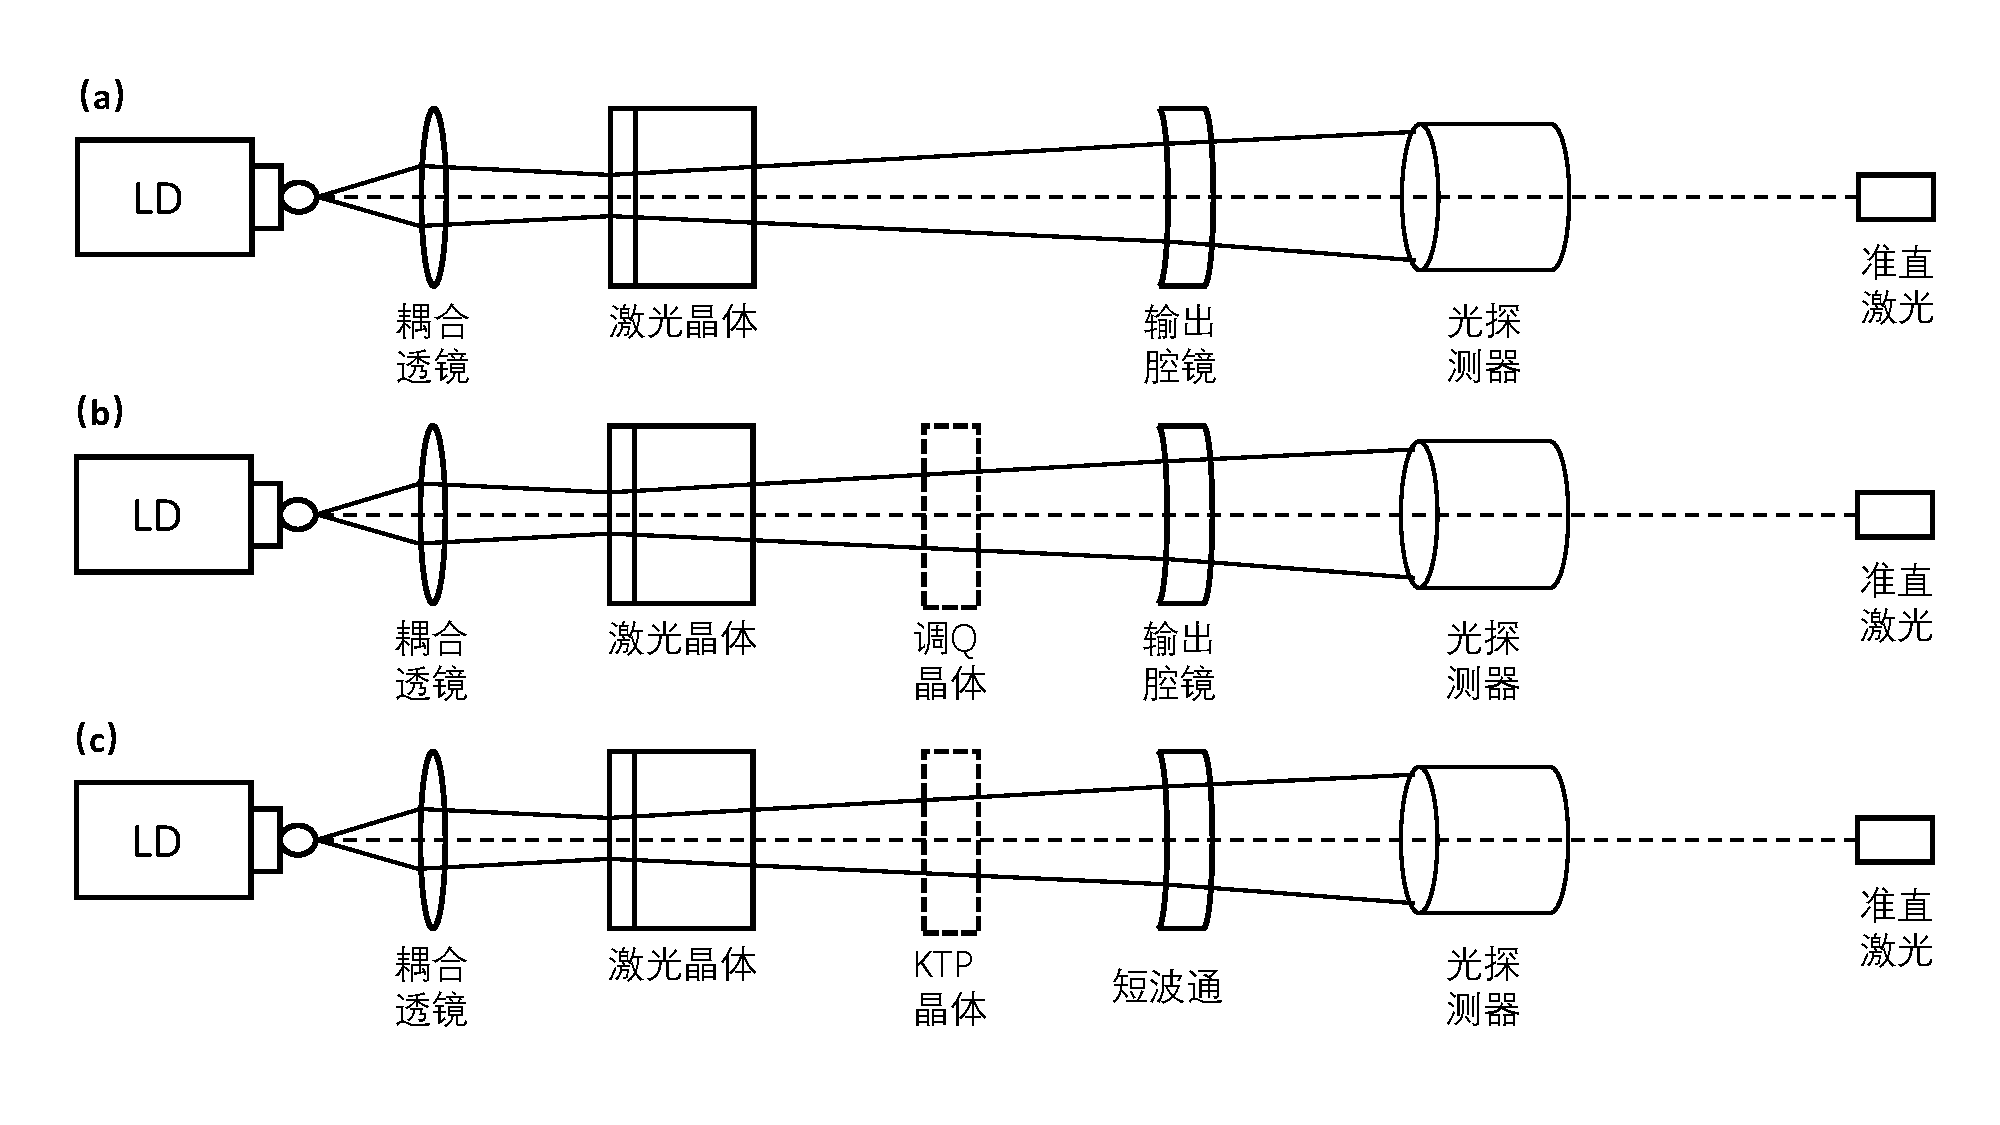
\includegraphics[width=0.95\linewidth]{fig/apparatus.pdf}
  \caption{实验装置示意图。(a)利用准直光搭建固体激光器示意图;(b)激光器的调Q光路示意图;(c)观测非线性二倍频效应的光路示意图。}
  \label{apparatus}
\end{figure}
\subsection{实验过程}
\subsubsection{测量LD激光工作特性}
打开光功率计和半导体泵浦激光器预热10分钟。预热完毕之后,将光功率计的探头置于半导体激光器的输出端口前,从电流0开始,缓慢调节电流并观察激光功率计实数,测量不同电流下LD激光器的功率,并且找到功率随电流开始显著变化的LD激光器工作电流阈值。
\subsubsection{搭建固体激光器并测量红外激光输出功率}
在光纤输出端前依次放上耦合透镜、激光晶体和输出镜。首先选用Nd:YVO$_4$晶体作为固体增益介质。

用红外相纸挡在固体激光器的输出端,缓慢调节LD激光器的工作电流到1.7 A左右,稍微晃动输出腔镜就可以在红外显示卡上捕捉到激光亮斑,这就是固体增益介质产生的1064 nm激光。微调输出腔镜的俯仰、倾角和位置,并且调整激光晶体(即Nd:YVO$_4$晶体)的位置,反复优化光路后使得光功率计读数达到极大值,此时对应的就是最佳输出(在1.7 A泵浦下功率达到300 mW左右)。随后改变泵浦电流大小,利用光功率计测量LD激光器工作电流阈值以上的激光功率随LD功率的变化。

随后将LD激光器电流降为0,并将晶体更换为Nd:YAG,重新按照之前的要求调整光路,测量测量LD激光器工作电流阈值以上的激光功率随LD功率的变化。
\subsubsection{被动调Q获得脉冲激光并观测脉冲激光输出特性}
将LD电流降为0,激光晶体选择Nd:YAG,在光学谐振腔中放入调Q晶体并调整位置,增大泵浦电流,用红外相纸在输出端可以观察到脉冲红外激光光斑(只有当激光晶体输出的激光的强度大于一定范围的时候,脉冲才可以被观察到)。用光功率计测量脉冲激光的平均功率。并用快速光电探测器观测调Q脉冲波形,测量不同泵浦功e率下,调Q脉冲的脉宽和重复率。
\subsubsection{利用KTP晶体产生非线性二倍频效应并观察}
将LD电流降为0,激光晶体选用Nd:YVO$_4$,并将输出镜换为短波通,在激光晶体与短波通之间放入倍频晶体(本实验我们使用KTP晶体)。适当调整短波通和KTP晶体的倾角、俯仰和距离(尽量靠近激光晶体),就可以观察到明亮的532 nm绿光。调整KTP晶体的倾角,使得输出的绿光最明亮(此时相位匹配成功),随后用光功率计测量输出功率随泵浦光功率的变化。
\section{实验结果与分析}
\subsection{LD激光工作特性}
测量得到808 nm泵浦激光的光功率和激励电流的关系曲线如图\ref{fig:PLD_I}所示。可以发现,在0.45 A左右,泵浦激光功率发生了明显的变化,因此可以判断阈值电流为0.45 A。在阈值之下,泵浦激光输出功率很低,几乎为0;在阈值电流以上,泵浦激光的光功率和激励电流呈线性关系,拟合结果给出
\begin{equation}\label{eq:PLD_I}
  P_{\rm LD}({\rm W})=0.68\times I_{\rm LD}({\rm A})-0.27,\quad r=0.9999.
\end{equation}
在之后的数据处理中,我们会用上面线性拟合给出的结果来计算特定激励电流下泵浦激光的功率。
\begin{figure}[h]
  \centering
  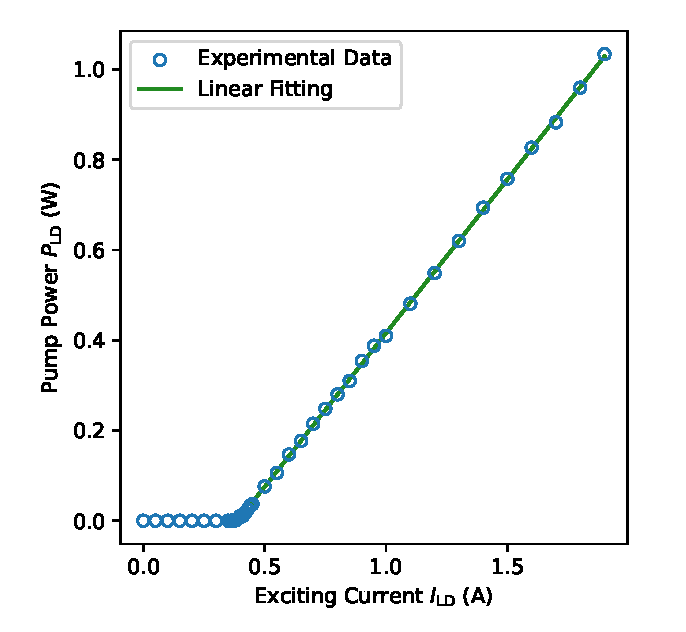
\includegraphics[width=0.6\linewidth]{fig/PLD_I.pdf}
  \caption{泵浦激光功率-激励电流关系图。阈值电流在0.45 A左右,在阈值电流之上,泵浦激光功率和激励电流基本呈线性关系,线性拟合的结果也在图中给出。}
  \label{fig:PLD_I}
\end{figure}
\subsection{红外激光输出功率随泵浦功率的关系}
仔细调节激光晶体的位置,使得输出激光功率最大。本实验中,对于Nd:YVO$_4$晶体,当激励电流为1.7 A时,输出激光功率最高调节到340 mW;对于Nd:YAG晶体,当激励电流为1.7 A时,输出激光功率最高调节到270 mW。测量得到两种晶体在不同泵浦光功率下的激光功率和转换效率如图\ref{fig:Plaser_PLD}所示。

可以看出,不论是Nd:YVO$_4$晶体还是Nd:YAG晶体,在本实验中的泵浦激光功率范围内,其激光功率都随着泵浦光功率呈线性变化。拟合结果给出
\begin{equation}\label{eq:Plaser_PLD}
  \begin{aligned}
    &{\rm Nd:YVO_4}&P_{\rm laser}({\rm W})=0.41\times P_{\rm LD}({\rm W})-0.022,\\
    &{\rm Nd:YAG}&P_{\rm laser}({\rm W})=0.33\times P_{\rm LD}({\rm W})-0.029.
  \end{aligned}
\end{equation}
从式\ref{eq:Plaser_PLD}中我们知道,相比于Nd:YAG晶体,Nd:YVO$_4$晶体激光功率随泵浦功率的增加而增加的速度更快,其效率也更高。而两种晶体的转换效率都随着泵浦光功率的增加而上升,最后有饱和的倾向。

在本实验的测量范围内,两种晶体在最佳工作状态下的最大转换效率分别为
\begin{equation}
  \begin{aligned}
    &{\rm Nd:YVO_4}&\eta_{\max}=40.0\%,\\
    &{\rm Nd:YAG}&\eta_{\max}=30.5\%.
  \end{aligned}
\end{equation}
\begin{figure}[h]
  \centering
  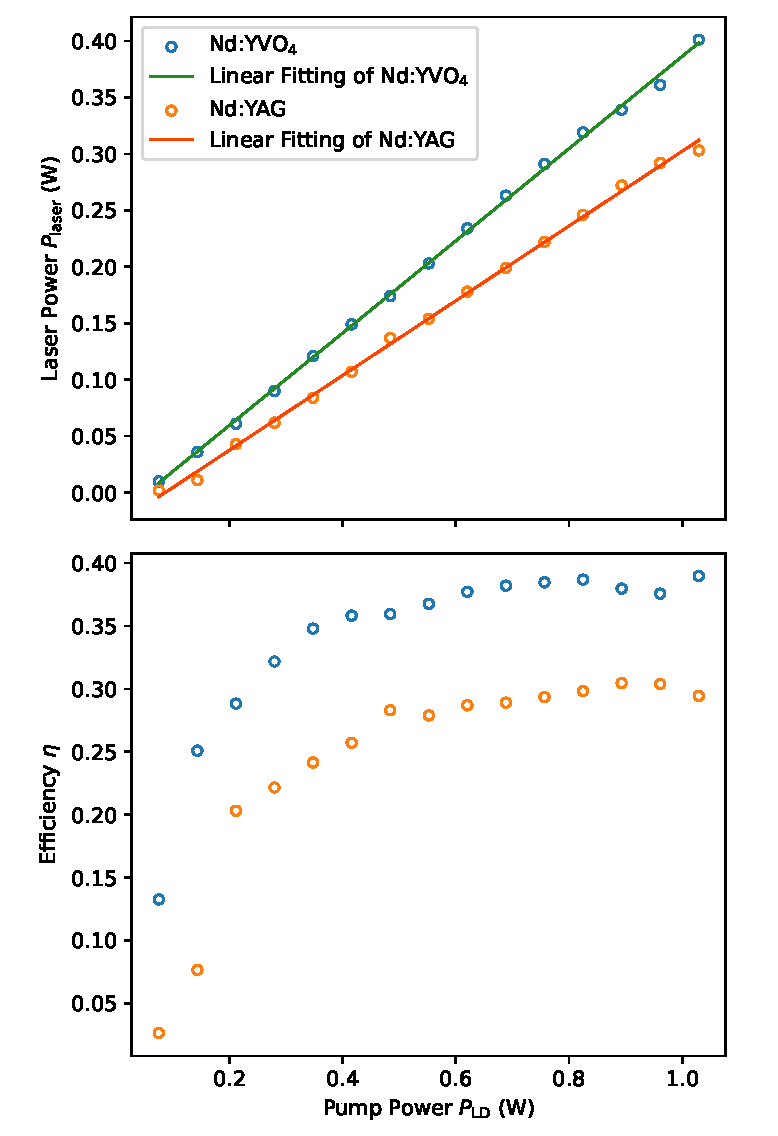
\includegraphics[width=0.6\linewidth]{fig/Plaser_PLD.pdf}
  \caption{两种晶体的激光功率随泵浦激光功率的变化关系图。不同激励电流下的泵浦激光功率是由线性拟合给出的结果计算得到的(见式\ref{eq:PLD_I})。两种晶体在本实验中的泵浦激光功率范围内,其激光功率都随着泵浦光功率呈线性变化。}
  \label{fig:Plaser_PLD}
\end{figure}
\subsection{被动调Q脉冲激光的输出特性}
晶体选用Nd:YAG。激励电流的阈值在1.25 A,在阈值电流之下,我们几乎观察不到脉冲激光,这是由于调Q晶体对于低光强有较强的吸收;而在阈值电流之上,脉冲激光的强度会发生一个突变,此时我们可以在红外相纸上观察到调Q脉冲激光。测量得到不同泵浦激光功率下脉冲激光的平均功率和转换效率如图\ref{fig:Ppulse_PLD}所示。

可以看到,在阈值电流(1.25 A)之上,两个激光的功率近似为线性关系,拟合结果给出
\begin{equation}
  P_{\rm pulse}({\rm mW})=152\times P_{\rm LD}({\rm W})-74.
\end{equation}并且在本实验的测量范围内,脉冲激光的转换效率随泵浦功率的增加不断提高。
\begin{figure}[h]
  \centering
  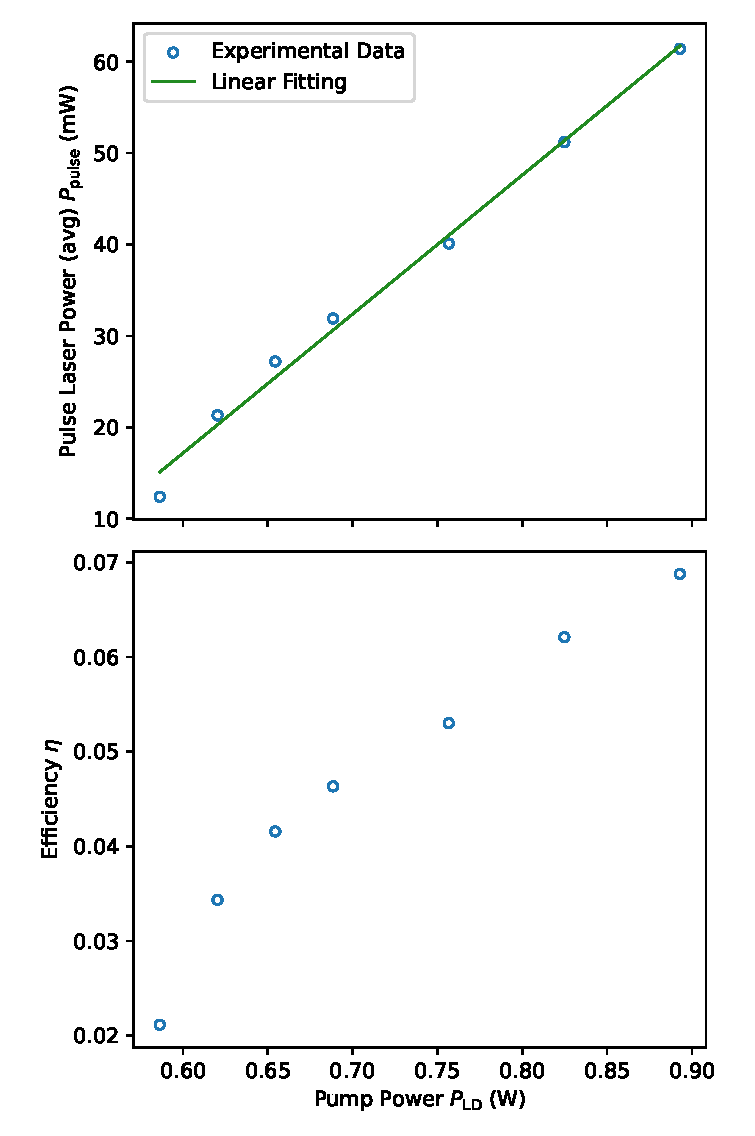
\includegraphics[width=0.6\linewidth]{fig/Ppulse_PLD.pdf}
  \caption{使用Nd:YAG晶体搭建的调Q脉冲激光功率随泵浦激光功率的变化关系图。不同激励电流下的泵浦激光功率是由线性拟合给出的结果计算得到的(见式\ref{eq:PLD_I})。在阈值电流(1.25 A)之上,两个激光的功率近似为线性关系,并且在本实验的测量范围内,脉冲激光的转换效率随泵浦功率的增加不断提高。}
  \label{fig:Ppulse_PLD}
\end{figure}

利用快速光电探测器,还可以观察脉冲激光的时间特性。使用Nd:YAG晶体调Q后输出的脉冲激光信号如图\ref{fig:pulse}所示。这个脉冲的宽度是非常窄的,也就说这个激光脉冲的性能是相对比较好的。利用示波器测量到的脉冲脉宽和重复率如表\ref{tab:Ppulse_PLD}所示。我们可以看出,对于Nd:YAG晶体,随着泵浦激光的功率增大,脉宽几乎不变,但重复率不断增加。
\begin{figure}[h]
  \centering
  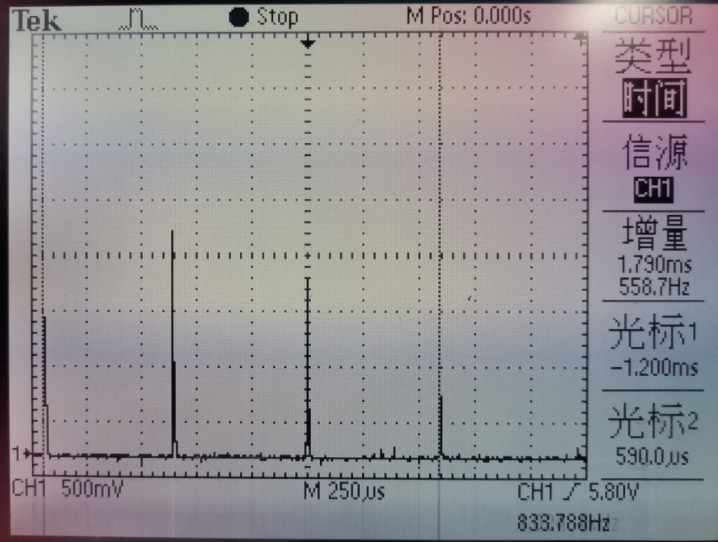
\includegraphics[width=0.5\linewidth]{fig/pulse.png}
  \caption{Nd:YAG晶体调Q后输出的脉冲激光信号}
  \label{fig:pulse}
\end{figure}
\begin{table}[h]
  \centering
  \caption{Nd:YAG晶体调Q产生的脉冲脉宽和重复率随激励电流的变化。脉冲宽度基本不随着激励电流的变化而变化,但是重复率随着激励电流的增加不断增加。}
  \label{tab:Ppulse_PLD}
  \setlength{\tabcolsep}{1cm}{
  \begin{tabular}{ccc}
    \hline\hline
  激励电流$I$ (A) & 脉冲宽度 (ns) & 重复率 (kHz)  \\\hline
  1.3  & 63   & 3.97 \\
  1.4  & 55   & 4.72 \\
  1.5  & 60   & 5.32 \\
  1.6  & 59   & 5.62 \\
  1.7  & 60   & 6.49 \\
  1.8  & 60   & 6.58 \\
  1.9  & 60   & 6.67 \\\hline\hline
  \end{tabular}}
\end{table}
\subsection{非线性二倍频效应}
晶体选用Nd:YVO$_4$。调节KTP晶体的角度至最佳输出处(见图\ref{fig:green}),利用光功率计测量二倍频光功率随基频光功率(也就是我们之前测量过的Nd:YVO$_4$晶体激光在不同激励电流下的功率)如图\ref{fig:P2w_Pw}所示。

从图\ref{fig:P2w_Pw}我们可以看到,二倍频信号的功率和基频信号的功率近似呈现二次函数关系,拟合结果给出
\begin{equation}
  P_{2\omega}({\rm mW})=84P_{\omega}^2({\rm W})+20P_{\omega}({\rm W}).
\end{equation}
这是符合我们的预期的,因为这是一个二级非线性效应,从式\ref{eq:2order}可以看到,二级的效应和基频的二次方成正比。
\begin{figure}[h]
  \centering
  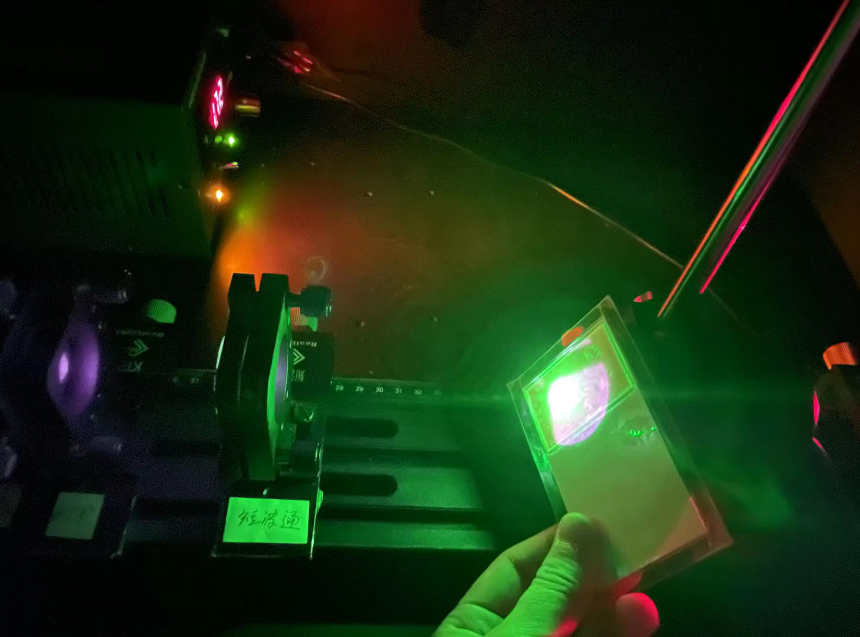
\includegraphics[width=0.5\linewidth]{fig/green.png}
  \caption{Nd:YVO$_4$晶体倍频后输出的绿色激光}
  \label{fig:green}
\end{figure}
\begin{figure}[h]
  \centering
  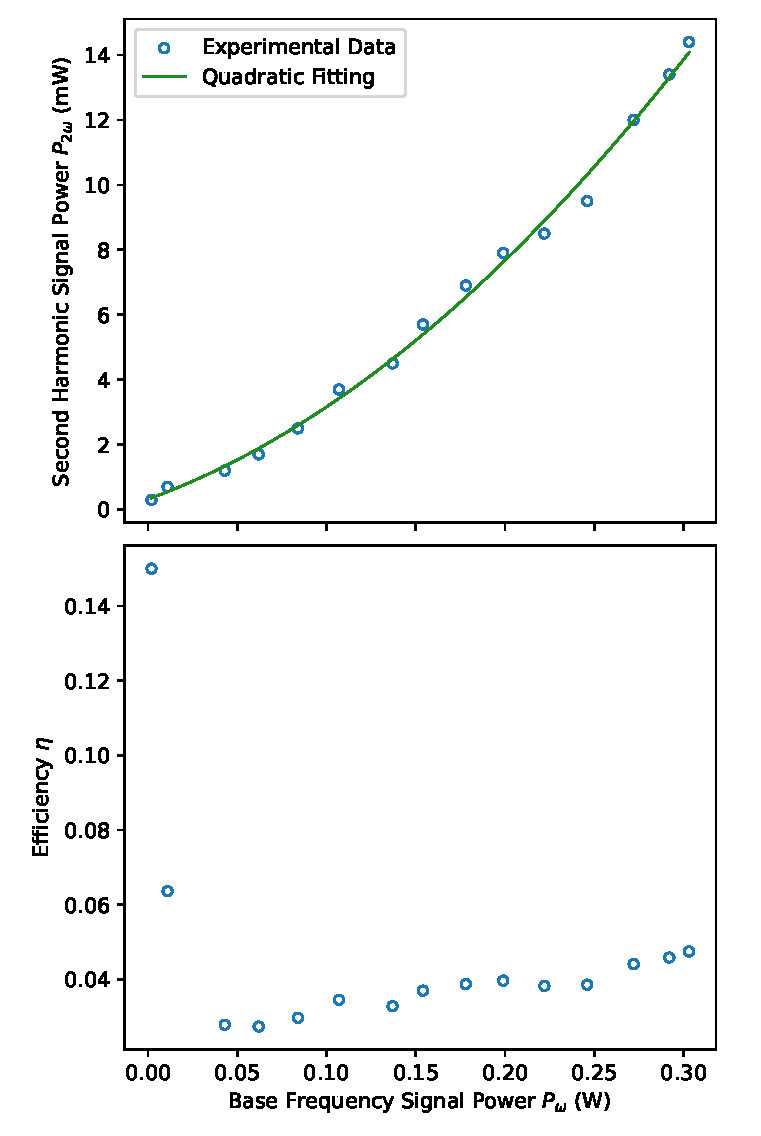
\includegraphics[width=0.6\linewidth]{fig/P2w_Pw.pdf}
  \caption{二倍频光功率和基频光功率关系图(激光晶体选用Nd:YVO$_4$)。图中我们使用了二次函数曲线拟合。}
  \label{fig:P2w_Pw}
\end{figure}
\section{结论}
通过实验,我们成功地利用808 nm半导体激光器、Nd:YVO$_4$晶体、Nd:YAG晶体、耦合透镜和输出腔镜等设备,组装出一台能稳定输出1064 nm激光的连续波固态激光器。其最大转换效率分别达到32.6\%(Nd:YVO$_4$晶体)和39.2\%(Nd:YAG晶体)。

我们还通过被动调Q获得了由Nd:YAG晶体激发的1064 nm脉冲激光,其最大转换效率约为7\%。随后,通过使用快速光电探测器和示波器,我们测量了脉冲激光的时间特性。研究发现,随着泵浦光功率的增加,脉冲激光的脉宽基本不变,而重复率增加。

此外,通过使用Nd:YVO$_4$、KTP晶体和短波通,我们获得并输出了532 nm的二倍频绿光。实验中,我们观察到了角度相位匹配对二倍频信号强度的影响,同时我们还测量了倍频转换效率与基频光功率,我们发现它们近似成二次方关系。
\begin{acknowledgments}
特别感谢刘开辉老师和黄琛学长在实验过程中的指导,尤其是黄学长在关键时候给我们的帮助,这使得我们能在规定时间内顺利的完成这个实验。感谢黄昊学长协力完成了本实验。
\end{acknowledgments}

\begin{thebibliography}{}
  \bibitem{wiki} “Laser”, Wikipedia. Nov. 03, 2023. [Online]. Available: https://en.wikipedia.org/w/index.php?title=Laser\&oldid=1183264651
  \bibitem{book} 吴思诚, 荀坤. 近代物理实验(第四版). 北京: 高等教育出版社, 2015.
  \bibitem{manual} 半导体激光泵浦固体激光调Q与光学二倍频实验仪器说明(实验室提供)
\end{thebibliography}
  
\clearpage % 附录前另起一页
\appendix % 附录开始
\section{思考题}
\subsection{LD泵浦固体激光器与氙灯泵浦的固体激光器相比有哪些优点?}
LD泵浦固体激光器具有体积小、重量轻、结构牢固、寿命长等诸多优点。

半导体激光器(LD)的发射阈值低,发射光谱可通过选择半导体材料和温度控制在宽范围内选择和精确调节。
\subsection{被动调Q使用的可饱和吸收体,其饱和光强不能太大,也不能太小,为什么}
若饱和光强过大,有可能全部的激光都被调Q晶体吸收,没有办法输出脉冲光。若饱和光强过小,输出激光脉冲的强度很小,而且脉冲展宽较宽(也就是一个扁平的“波包”),甚至有可能输出连续波。
\subsection{光学二倍频只能在非中心对称的介质中进行,为什么?}
由于二阶电极化强度是一个三阶张量,只有无对称中心的晶体才有可能使其三阶张量的分量全不为零。具有中心反演对称性的介质,其二阶(其实是所有偶数阶)非线性极化率张量均为0,因此光学二倍频不能在具有中心对称的介质中进行。
\subsection{若在激光腔内再放置一块晶体,造成$\omega$光与$2\omega$光的和频,其相位匹配条件是什么?}
相位匹配条件是根据光子的动量守恒得到的
\begin{equation}
  \bm{k_1}+\bm{k_2}=\bm{k_3},
\end{equation}
其中$\bm{k_1},\bm{k_2},\bm{k_3}$分别对应频率为$\omega,2\omega,3\omega$的光波波矢。于是我们有
\begin{equation}
  k_i=\frac{n^{(\omega_i)}\omega_i}{c}.
\end{equation}
那么相位匹配要求
\begin{equation}
  n^{(\omega)}+n^{(2\omega)}=n^{(3\omega)}.
\end{equation}
\section{实验记录本}
实验记录本。
\end{document}
